\section{Decision Trees}

Next, we trained a single decision tree classifier on the training dataset, see \autoref{fig:decision_tree}. Using a simple search of numerous values we set max-depth to $3$, which worked well. The model achieves the score of $87.7\%$ in training and $78.3\%$ on the test dataset.

\begin{figure*}
    \centering
    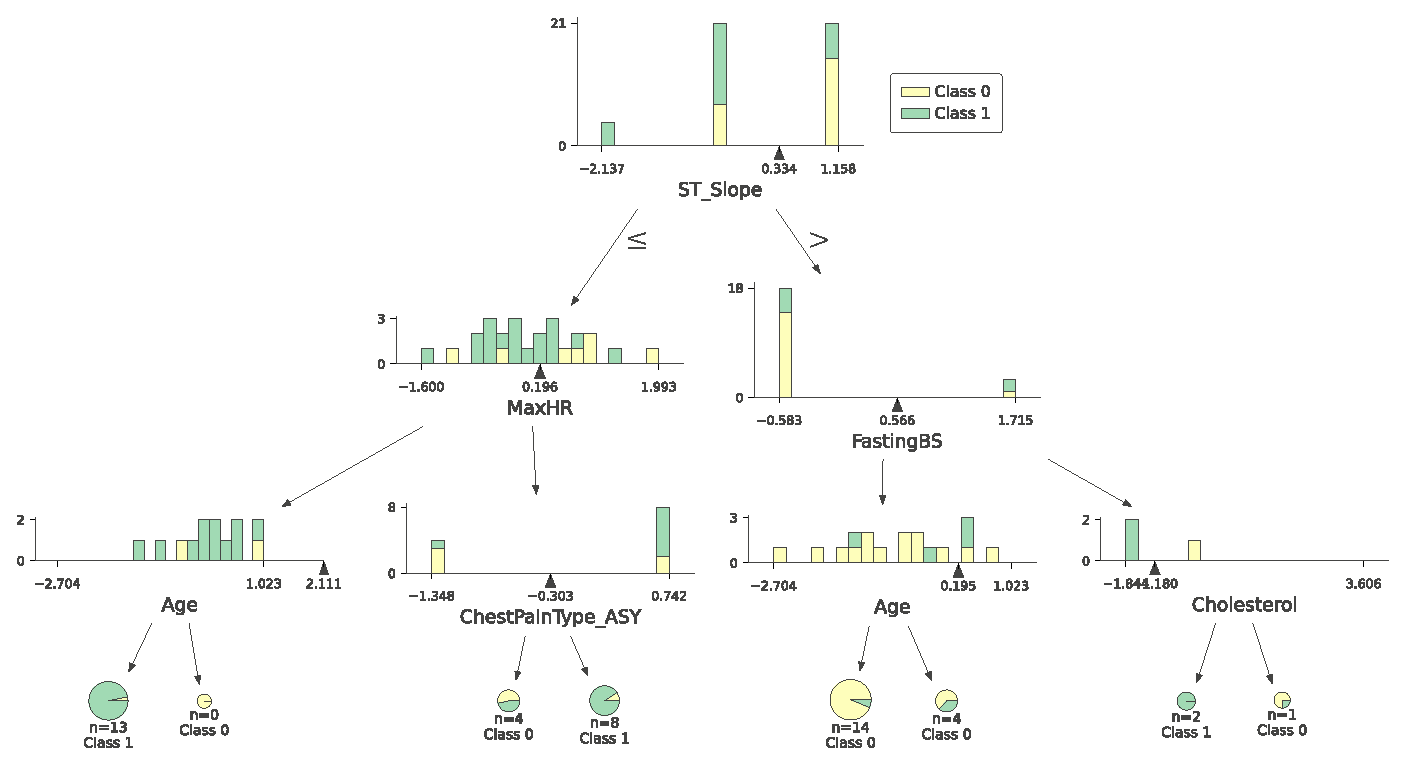
\includegraphics[width=1\textwidth]{images/decision_tree.pdf}
    \caption{A visualization of the trained decision tree.}
    \label{fig:decision_tree}
\end{figure*}

\begin{figure}
    \centering
    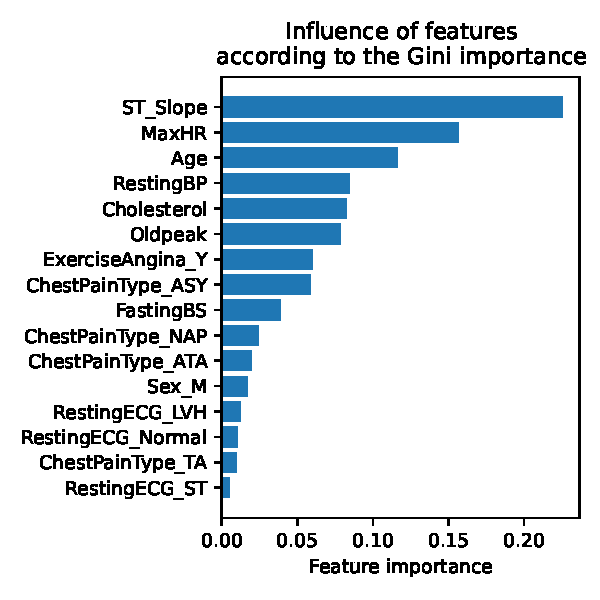
\includegraphics[width=1\columnwidth]{images/random_forest.pdf}
    \caption{A visualization of the influence of the
different features according to the Gini importance.}
    \label{fig:random_forest}
\end{figure}

Further, we trained a random forest classifier using an ensemble of 100 decision trees. In this case, the training data could be learned perfectly, and the achieved test score was $80.4\%$, demonstrating an improvement against a single decision tree.

We visualized the Gini importance of the features in \autoref{fig:random_forest}.

